%%%%%%%%%%%%%%%%%%%%%%%%%%%%%%%%%%%%%%%%%%%%%%%%%%%%%%%%%%%%%%%%%%%%%%%%%%

% abnTeX2: Modelo de Trabalho Acadêmico em conformidade com 
% as normas da ABNT

%%%%%%%%%%%%%%%%%%%%%%%%%%%%%%%%%%%%%%%%%%%%%%%%%%%%%%%%%%%%%%%%%%%%%%%%%%

\documentclass[english, 
               brazil, 
               bsc] %Opções bsc (TCC) e msc (Mestrado)
               {dcomp-abntex2}


%%%%%%%%%%%%%%%%%%%%%%%%%%%%%%%%%%%%%%%%%%%%%%%%%%%%%%%%%%%%%%%%%%%%%%%%%%
% Área para adição de pacotes extras
%%%%%%%%%%%%%%%%%%%%%%%%%%%%%%%%%%%%%%%%%%%%%%%%%%%%%%%%%%%%%%%%%%%%%%%%%%

\usepackage{lipsum} %Retirar para a versão final do documento

%Utilize aqui seu pacote preferido para algoritmos
\usepackage[linesnumbered]{algorithm2e}

%%%%%%%%%%%%%%%%%%%%%%%%%%%%%%%%%%%%%%%%%%%%%%%%%%%%%%%%%%%%%%%%%%%%%%%%%%

%Compila o indice
\makeindex

\begin{document}

% Seleciona o idioma do documento (conforme pacotes do babel)
\selectlanguage{brazil}

% Retira espaço extra obsoleto entre as frases.
\frenchspacing 

%%%%%%%%%%%%%%%%%%%%%%%%%%%%%%%%%%%%%%%%%%%%%%%%%%%%%%%%%%%%%%%%%%%%%%%%%%
% ELEMENTOS PRÉ-TEXTUAIS
%%%%%%%%%%%%%%%%%%%%%%%%%%%%%%%%%%%%%%%%%%%%%%%%%%%%%%%%%%%%%%%%%%%%%%%%%%

\pretextual

% \titulo{Desenvolvendo aplicações com arquitetura de microserviços usando o framework DevOps} 
\titulo{Padrões de desenvolvimento de aplicações com arquitetura de microserviços da perspectiva da cultura DevOps} 
\autor{João Paulo Feitosa Secundo}
\orientador{Rafael Oliveira Vasconcelos}
\coorientador{}
\curso{Ciência da Computação}

\inserirInformacoesPDF

\imprimircapa
\imprimirfolhaderosto*

% \include{Pre_Textual/Dedicatoria}
% \begin{agradecimentos}

Teste agradecimentos

\end{agradecimentos}
% ---
% \include{Pre_Textual/Epigrafe}
% % resumo em português
\setlength{\absparsep}{18pt} % ajusta o espaçamento dos parágrafos do resumo
\begin{resumo}

O presente trabalho analisa o desenvolvimento de aplicações com arquitetura de microsserviços, expondo as características desta abordagem arquitetural e reunindo e discutindo práticas usadas no desenvolvimento de aplicações que a usa, por meio de pesquisa e revisão bibliográfica. Também serão discutidas e usadas algumas ferramentas para o desenvolvimento de uma aplicação de exemplo. O resultado é um conjunto de características comuns, práticas bem consolidadas e ferramentas úteis no desenvolvimento de tais aplicações. Ademais, foi identificado que certas práticas têm circunstâncias subjetivas e devem ser ponderadas antes de aplicadas, pois nem sempre são consideradas favoráveis, por vezes sendo julgadas positivas por alguns autores e negativas por outros.

% Ademais, foi identificado certo nível de discordância entre autores respeitados nesta área sobre a prática de começar a aplicação por uma abordagem arquitetural mais simples, tal como a monolítica, antes de adotar os microsserviços, questão em que há mais espaço para discussões e estudos de caso. 

% Segundo a \citeonline[3.1-3.2]{NBR6028:2003}, o resumo deve ressaltar o objetivo, o método, os resultados e as conclusões do documento. A ordem e a extensão destes itens dependem do tipo de resumo (informativo ou indicativo) e do tratamento que cada item recebe no documento original. O resumo deve ser precedido da referência do documento, com exceção do resumo inserido no próprio documento. (\ldots) As palavras-chave devem figurar logo abaixo do resumo, antecedidas da expressão Palavras-chave:, separadas entre si por ponto e finalizadas também por ponto.

 \textbf{Palavras-chave}: arquitetura de \emph{software}. microsserviços. desenvolvimento. práticas. ferramentas.
\end{resumo}
% % resumo em inglês
\setlength{\absparsep}{18pt} % ajusta o espaçamento dos parágrafos do resumo
\begin{resumo}[Abstract]
 \begin{otherlanguage*}{english}
   This paper analyzes the development of applications with microservice architecture, exposing the characteristics of this architectural approach and gathering and discussing practices used in the development of applications that use it, through literature research and review. Some tools will also be discussed and used for the development of an example application. The result is a set of common characteristics, well established practices and useful tools in the development of such applications. Furthermore, it has been identified that certain practices have subjetive circumstances and must be pondered before applied, for they are not always considered favorable, sometimes being judged positive by some authors and negative by others.
   
  %  it has been identified a certain level of disagreement between respected authors in this area about the practice of starting with a simpler architectural approach, such as the monolithic one, before utilizing microservices, issue in which there is more space for discussions and case studies.

   \vspace{\onelineskip}
 
   \noindent 
   \textbf{Keywords}: software architecture. microservices development. practices. tools.
 \end{otherlanguage*}
\end{resumo}


% \mostrarlistadeILUSTRACOES
% \mostrarlistadeQUADROS
% \mostrarlistadeTABELAS
% \mostrarlistadeCODIGOS
% \mostrarlistadeALGORITMOS
 
% Lista de abreviaturas e siglas

\begin{siglas}
	\item[API]{Application Programing Interface - Interface para programação de aplicação}
	\item[HTTP]{HyperText Transfer Protocol - Protocolo de transferência de hipertexto}
	\item[AMS]{Arquitetura de microsserviços}
	\item[DoS]{Denial of Service - Negação de serviço}
	\item[RFC]{Request For Comments - Pedido de comentários}
	\item[JSON]{JavaScript Object Notation - Notação de objeto javaScript}
	\item[DDD]{Domain-driven Design - Projeto orientado a domínio}
	\item[SSL]{Secure Socket Layer - Camada de soquete seguro}
\end{siglas}
% \include{Pre_Textual/Simbolos}
    
\mostrarSUMARIO

%%%%%%%%%%%%%%%%%%%%%%%%%%%%%%%%%%%%%%%%%%%%%%%%%%%%%%%%%%%%%%%%%%%%%%%%%%
% ELEMENTOS TEXTUAIS
%%%%%%%%%%%%%%%%%%%%%%%%%%%%%%%%%%%%%%%%%%%%%%%%%%%%%%%%%%%%%%%%%%%%%%%%%%

\textual
\chapter{Introdução}\label{chapter-introducao}

O crescimento da Internet e a onipresença da computação móvel tem mudado o jeito como \emph{software} é desenvolvido nos últimos tempos. Todos que têm contato com a área do desenvolvimento de \emph{software} provavelmente conhecem o termo \emph{SaaS (Software as a Service)}, ou \emph{software} como um serviço. Entretanto, essa expressão significa mais do que apenas um modelo de negócio. A tendência que tem-se observado na indústria do \emph{software} é a de oferecer \emph{software} não mais como um pacote completo e fechado, mas sim como um pacote flexível e em constante melhoria, o que implica na mudança do foco dos desenvolvedores para a criação de aplicações modulares, e que permitam que mudanças sejam desenvolvidas e implantadas rápida, fácil e independentemente \cite{CAOPLE, oracle_microservices}.

Essa mudança de foco implicou no surgimento de novas abordagens de arquitetura e organização de \emph{software}, e uma dessas tem ganho grande popularidade na indústria do \emph{software} por facilitar a criação de aplicações que são multilíngues, facilmente mantidas e implantadas, escaláveis, e altamente disponíveis. Inspirada na arquitetura orientada a serviços, ela se chama arquitetura de microsserviços, e é considerada por muitos profissionais da engenharia de \emph{software} como a melhor maneira de arquitetar uma aplicação de \emph{software} como um serviço atualmente. Entretanto, como tudo na computação, há um \emph{trade-off} (uma troca), pois assim como há benefícios, também há desvantagens e desafios no emprego de uma arquitetura de microsserviços, os quais também são discutidos neste trabalho \cite{middleware-microservices,design-monitoring-testing-waseem}.


% Many development teams have found the microservices architectural style to be a superior approach to a monolithic architecture. But other teams have found them to be a productivity-sapping burden. Like any architectural style, microservices bring costs and benefits. To make a sensible choice you have to understand these and apply them to your specific context. microservice tradeoffs - https://martinfowler.com/articles/microservice-trade-offs.html#summary

%Se você quiser projetar um aplicativo que seja multilíngue, facilmente escalável, fácil de manter e implantar, altamente disponível e que minimize falhas, use a arquitetura microservices para projetar e implantar um aplicativo em nuvem. Em uma arquitetura de microservices, cada microservice possui uma tarefa simples e se comunica com os clientes ou com outros microservices usando mecanismos de comunicação leves, como solicitações de API REST. \cite{oracle_microservices}

% O público alvo e os usuários desses softwares podem chegar a números imensos.

% In recent years, the rise of the internet and the ubiquity of mobile computing have made it necessary for application developers to design their applications focusing on a lightweight, self-contained component. Developers need to deploy applications quickly and make changes to the application without a complete redeployment. This has led to a new development paradigm called "microservices," where an application is broken into a suite of small, independent units that perform their respective functions and communicate via APIs. Although independent units, any number of these microservices may be pulled by the application to work together and achieve the desired results. \cite{middleware-microservices}

%For the past several years, we have been developing standards and practices for team development of large, complex systems using a layered, monolithic architecture. This is reflected in how we organize into teams, structure our solutions and source code control systems, and package and release our software.

% ---
\section{Objetivos}\label{sec-objetivos}
% ---

% Esta seção descreve os objetivos do trabalho. Esta é a \autoref{sec-objetivos}. Veja os objetivos específicos em \autoref{sec-objetivos-especificos}.

\subsection{Objetivo geral}\label{sec-objetivo-geral}

Analisar o desenvolvimento de aplicações com arquitetura de microsserviços.
% , discutindo boas práticas e ferramentas comumente usadas.
% Analisar e resumir o estado da arte em desenvolvimento de aplicações com arquitetura de microsserviços

\subsection{Objetivos específicos}\label{sec-objetivos-especificos}

% (TCC 1:)
- Caracterizar a arquitetura de microsserviços;
% - Apresentar? e caracterizar a arquitetura de microsserviços;

- Apresentar e discutir práticas comumente usadas no desenvolvimento de aplicações com arquitetura de microsserviços;
% - Apresentar? e discutir práticas comumente usadas no desenvolvimento de aplicações com arquitetura de microsserviços;

% - Analisar a viabilidade da aplicação a ser desenvolvida no TCC 2

% (TCC 2:)
% Analisar a eficiência dessas boas práticas;
% - Analisar/testar a eficiência desses padrões e práticas, por meio de (estudos de caso? análise da literatura? exemplos de empresas que as usam?);

% \textbf{Reescrever esse objetivo:}
% \sout{- Propor uma combinação de ferramentas para o desenvolvimento de aplicações com arquitetura de microsserviços;}

% \textbf{Pode ser reescrito como: }
% \sout{- Demonstrar uma combinação de ferramentas sendo usada em uma aplicação real com arquitetura de microsserviços, e possíveis alternativas}

% \textbf{Ou então:}
% \sout{- Propor uma combinação de ferramentas open-source ou gratuitas para o desenvolvimento de app com arq de microsserviços}

% Vai ser reescrito como:
- Apresentar ferramentas que são frequentemente usadas e que cumprem propósitos importantes em aplicações com arquitetura de microsserviços;
% Objetivo mais específico: Expor uma boa quantidade de ferramentas tal que supra as necessidades mais básicas/frequentes de uma arquitetura de microsserviços, com algumas alternativas.

- Contextualizar essas ferramentas, apontando os problemas que resolvem e necessidades que suprem, assim como seus pontos positivos e negativos;
% - Contextualizar essas ferramentas COMPARATIVAMENTE, apontando os problemas que resolvem e necessidades que suprem;

- Desenvolver uma aplicação exemplar com arquitetura de microsserviços, usando uma combinação das ferramentas e práticas apresentadas;

% \textbf{Será que dá pra apontar pontos positivos e negativos de todas as ferramentas apresentadas? Talvez seja melhor apontar apenas os das ferramentas usadas..:}
% - Apontar pontos positivos e negativos das ferramentas usadas na aplicação exemplar.


\section{Metodologia}

Para o desenvolvimento deste trabalho, inicialmente foi feita uma pesquisa exploratória sobre a arquitetura de microsserviços, com o objetivo de ganhar maior familiaridade com o tema. Depois de definidos os objetivos, foi iniciada uma pesquisa bibliográfica e os trabalhos mais relevantes foram filtrados e estudados. Os trabalhos julgados como mais relacionados ao tema tratado foram estudados mais a fundo e, com assistência dos modelos de inteligência artifical GPT-3.5 e GPT-4, foram resumidos para serem apresentados no capítulo de trabalhos relacionados.

Como foi constatado que não existe uma definição formal para a arquitetura de microsserviços, para caracterizá-la e para reunir práticas, foram extraídas dos trabalhos estudados as características ou práticas que apareceram com frequência ou que foram mencionadas como imprescindíveis pelos autores. Em seguida, essas características e práticas foram estudadas para então serem apresentadas de forma contextualizada, coesa e coerente neste trabalho.

%  apresentá-las essas práticas de maneira coesa do texto, também foi usada o GPT 3.5 e 4.5 para conexão de pontos-chave ideias   

%As boas práticas que abordavam questões de código profundamente foram desconsideradas por serem extensas e específicas.

% apenas boas práticas relacionadas a infraestrutura foram consideradas?

Para apresentar e contextualizar as ferramentas frequentemente usadas em aplicações com arquitetura de microsserviços, uma nova pesquisa bibliográfica foi feita para conhecer e extrair as mais comumente usadas. Após isso, algumas dessas ferramentas e das práticas mencionadas anteriormente foram escolhidas para serem usadas no desenvolvimento da aplicação exemplar, de acordo com as necessidades resultantes da escolha do domínio dessa e tendo em mente os limites do contexto do desenvolvimento deste trabalho acadêmico.

Depois de grande parte da aplicação ser desenvolvida, com o novo conhecimento adquirido a partir dessa experiência prática de desenvolvimento, de bastantes pesquisas bibliográficas, e também de consultas aos modelos de inteligência artifical GPT-3.5 e GPT-4, foi escrita a parte do trabalho que apresenta ferramentas para o desenvolvimento de microsserviços. Por fim, depois de finalizada a aplicação exemplar, foram elaborados os diagramas apropriados para então ser desenvolvida a parte do trabalho que a apresenta.

% com o objetivo de se entender como funcionam, os problemas que resolvem, suas vantagens e seus limites

% disso Após isso elas foram estudadas por pesquisa bibliográfica e com a ajuda dos modelos de inteligência artifical GPT 3.5 e GPT 4.5, com o objetivo de se entender como funcionam, os problemas que resolvem, suas vantagens e seus limites. Para apresentá-las no texto, os pontos-chave foram reunidos 

%Durante o desenvolvimento, foram reunidos pontos positivos e negativos observados no uso das ferramentas.  
 

% (metodologia quanto aos objetivos, quanto a execução. passo a passo que vai seguir durante o trabalho. explicar como analisar/testar essa eficiencia (objetivos especificos))

% pesquisa bibliográfica refere-se ao ato de reunir os materiais
% a revisão bibliográfica refere-se ao ato de estudar os materiais e extrair aquilo que interessa
\chapter{Fundamentação teórica}\label{chapter-fundamentacao}

\chapterprecis{Este capítulo aprensenta uma introdução sobre as arquiteturas de monolito e de microsserviços, e investiga trabalhos relacionados.}\index{sinopse de capítulo}

\section{As aplicações monolíticas}

Aplicações monolíticas, também chamadas de monólitos, são aplicações que possuem as camadas de acesso aos dados, de regras de negócios, e de interface de usuário em um único programa em uma única plataforma. Os monólitos são autocontidos e totalmente independentes de outras aplicações. Eles são feitos não para uma tarefa em particular, mas sim para serem responsáveis por todo o processo para completar determinada função. Em outras palavras, as aplicações monolíticas têm problema de modularidade. Elas podem ser organizadas das mais variadas formas e fazer uso de padrões arquiteturais, mas são limitadas em muitos outros aspectos, citados na \autoref{subsection-monolitos-limitacoes}.

\subsection{Benefícios}

O maior e melhor benefício da arquitetura monolítica é sua simplicidade. Uma aplicação simples é uma aplicação fácilmente entendida pelos seus desenvolvedores, o que melhora sua manutenibilidade. Para aplicações com um domínio simples, como um e-commerce de calçados por exemplo, optar por uma arquitetura complexa como a de microsserviços significaria adicionar uma enorme complexidade - provavelmente desnecessária - em seu desenvolvimento e infraestrutura.

Outra vantagem dos monolitos é sua facilidade de construção, tanto em relação a sua infraestrutura quanto ao seu desenvolvimento. Dentre todos os tipos de arquitetura, os monólitos têm o tipo de infraestrutura mais fácil de se construir, e além disso, neles geralmente não é necessário haver comunicação entre diferentes serviços ou máquinas, então os desenvolvedores não precisarão se preocupar com a complexidade que acompanha essa comunicação.

Até certo tamanho, são fáceis de manter porque são fáceis de serem entendidos. Porém, depois de crescer excessivamente, um monólito pode se tornar um emaranhado complexo de funcionalidades que são difíceis de diferenciar, de separar, e de manter. E então começam a surgir as limitações deles...

\subsection{Limitações}\label{subsection-monolitos-limitacoes}

As limitações das aplicações monolíticas incluem:

Crescimento, velocidade de desenvolvimento, e manutenção - Depois de chegar num certo tamanho, torna-se muito difícil desenvolver funcionalidades novas, ou mesmo prover manutenção às já existentes. Padrões de organização podem amenizar a situação, mas não eliminam o problema.

Confiabilidade - 

Escalabilidade -

Reutilização - 

Implantação - Necessidade de compilar toda a aplicação, mesmo as partes em que não houve mudanças, a cada implantação.

Resiliência - Falhas relativamente pequenas podem prejudicar toda a aplicação, mesmo as partes que não tiveram relação com a falha.

Flexibilidade - As escolhas de tecnologias são mais limitadas. Um projeto tende a usar apenas 1 solução devido a problemas de complexidade ou compatibilidade que podem surgir ao usar mais.

% ---
\section{Os microsserviços}
% ---

\begin{figure}[htb]
	\caption{\label{figura_arquitetura_microsservicos}Aplicação com arquitetura de microsserviços}
	\begin{center}
	    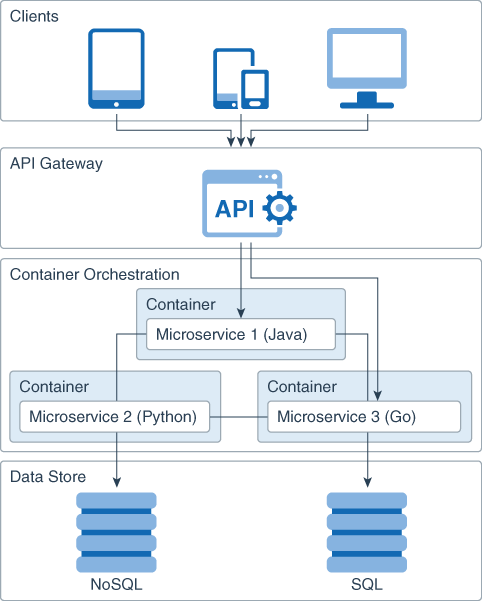
\includegraphics[scale=0.5]{Imagens/microservice_architecture.png}
	\end{center}
	\legend{Fonte: \citeonline{oracle_microservices}}
\end{figure}

Aplicações com uma arquitetura de microsserviços são separadas em partes, chamadas de microsserviços, que são classificadas e se comunicam por meio de uma rede. Microsserviços oferecem capacidades de negócio (funcionalidades relacionadas às regras de negócio da aplicação) ou capacidades de plataforma (funcionalidades relacionadas ao ambiente de execução da aplicação), tratando um aspecto em particular da aplicação. Eles se comunicam por meio de APIs bem definidas, contratos de dados, e configurações. O "micro" em microsserviços faz referência não ao tamanho do serviço, mas sim ao seu escopo de funcionalidade. Eles oferecem apenas uma determinada funcionalidade, tornando-se especialistas nela. Assim sendo, microsserviços não necessariamente devem ser pequenos em tamanho, mas fazem apenas uma tarefa e a fazem eficientemente. 
 
Sendo especialistas em apenas uma tarefa, microsserviços têm características e comportamentos que os diferenciam de outras arquiteturas orientadas a serviços, os quais serão discutidos no \autoref{chapter-caracteristicas}.

A \autoref{figura_arquitetura_microsservicos} exemplifica uma aplicação com arquitetura de microserviços. Inicialmente os usuários da aplicação (camada \emph{Clients}) fazem requisições à api para obter as informações desejadas. O \emph{API Gateway} - que é reponsável por integrar os serviços e será melhor discutido no \autoref{chapter-boas-praticas} - fará as devidas requisições para os devidos microsserviços (localizados na camada \emph{Container Orchestration}). Esses microsserviços então buscarão a informação necessária no devido banco de dados (camada \emph{Data Store}).

% A ilustração mostra as camadas da arquitetura de microsserviços. A primeira camada é a camada do cliente, que contém: os computadores, laptops e dispositivos móveis. A segunda camada é a camada do gateway de API, que redireciona as solicitações do cliente para os microsserviços apropriados. A terceira camada é a camada de orquestração de contêineres, com todos os microsserviços agrupados dentro de uma orquestração de contêineres. Cada um dos microsserviços está em contêiner. Eles se comunicam com os clientes por meio do gateway de API. A quarta camada é a camada de armazenamento de dados. Cada um dos microsserviços em contêiner que implementam persistência se comunica a apenas um armazenamento de dados. Os armazenamentos de dados exibidos são NoSQL e SQL.


% Microsserviços são uma abordagem arquitetônica e organizacional do desenvolvimento de software na qual o software consiste em pequenos serviços independentes que se comunicam usando APIs bem definidas. Esses serviços pertecem a pequenas equipes autossuficientes.

% A arquitetura de microsserviços (AMS) está ganhando força no desenvolvimento e entrega de aplicações de software como um conjunto de pequenos serviços granulares que podem ser integrados por meio de mecanismos de comunicação leve, normalmente APIs RESTful [10]. Microsserviços são componentes pequenos e facilmente entendíveis que possuem capacidades de negócio no meio dos serviços [11]. Esses serviços podem ser escalados independentemente (já que são desacoplados) pela implementação de \texttt{stacks} de tecnologias diferentes [2]. Muitos pesquisadores e praticantes dizem que AMS é uma evolução da Arquitetura orientada a serviços (AOS), como visto no contexto de serviços independentes/auto-suficientes e de natureza leve [12]. Por outro lado, AMS pode ser diferenciada da AOS em termos de compartilhamento de componentes, comunicação de serviços, mediação de serviços, e acesso remoto aos serviços [13]. (Bar, f., 2018, tradução nossa). \cite{WASEEM2020110798}
% % AOS é construida com base na ideia de compartilhar o máximo possível, enquanto AMS, o mínimo possível [13, 14]. AMS usa um estilo coreografico para comunicação inter-serviços, enquanto AOS aplica um estilo de orquestração para coordenação de serviços. Para mediação de serviços, AMS usa a camada de API que atua como uma fachada para o serviço, enquanto AOS adota o conceito de um \texttt{middleware} mensageiro para coodenação de serviços. Além disso, AMS em grande parte depende do protocolo REST e mensageria simples como protocolo de acesso remoto ao serviço; entretanto, AOS consegue lidar com diferentes tipos de protocolo de acesso remoto, incluindo mensageria simples para acessar serviços remotos [13].

\section{Trabalhos relacionados}

\subsection{{Microservices, IoT and Azure, por Bob Familiar - capítulo 2: What is a microservice}}

O capítulo 2 do livro de Bob Familiar descreve o que é um microsserviço, suas características e implicações, benefícios, e desafios. 

"Microservices do one thing and they do it well". Como é explicado por \citeonline{Familiar2015} , microsserviços representam business capabilities definidos usando o design orientado a domínio, são testados a cada passo do \emph{pipeline} de implantação, e lançados por meio de automação, como serviços independentes, isolados, altamente escaláveis e resilientes em uma infraestrutura em núvem distribuída. Pertecem a um time único de desenvolvedores, que trata o desenvolvimento do microsserviço como um produto, entregando software de alta qualidade em um processo rápido e iterativo com envolvimento do cliente e satisfação como métrica de sucesso.

\subsection{A Systematic Mapping Study on Microservices Architecture in DevOps, por Waseem, M., Liang, P. e Shahin, M.}

Esse trabalho tem o objetivo de sistematicamente identificar, analisar, e classificar a literatura sobre microsserviços em DevOps.

Inicialmente o leitor é contextualizado no mundo dos microsserviços e a cultura DevOps. Os autores usam a metodologia de pesquisa de um estudo de mapeamento sistemático da literatura publicada entre Janeiro de 2009 e Julho de 2018. Após selecionados 47 estudos, é feita a classificação deles de acordo com os critérios definidos pelos autores, e então é feita a discussão sobre os resultados obtidos - são expostos a quantidade de estudos sobre determinados tópicos em microsserviços, problemas e soluções, desafios, métodos de descrição, design patterns, benefícios, suporte a ferramentas, domínios, e implicações para pesquisadores e praticantes.

Os principais resultados são: (1) São identificados Três temas de pesquisa em AMS com DevOps “desenvolvimento e operações de microsserviços em DevOps”, “abordagens e suporte a ferramentas para sistemas baseados em AMS em DevOps”, e “Experiência de migração de AMS em DevOps”. (2) São identificados 24 problemas e apontadas suas respectivas soluções com respeito a implementação de microsserviços com DevOps. (3) A AMS é descrita princiapalmente usando caixas e linhas. (4) A maioria das qualidades da AMS são afetadas positivamente quando aplicadas com DevOps. (5) 50 ferramentas que suportam a construção de sistemas baseados em AMS são apontados. (6) A combinação da AMS e DevOps tem sido aplicada em uma ampla variedade de domínios de aplicações.


(Comparar cada trabalho com o meu trabalho. Coisas que eles não abordam e que eu abordo)

\chapter{Desenvolvimento}

Para provisionamento, considerar a ferramenta ~~

Para lançamento, considerar a tecnologia ~~

Para comunicação entre serviços, APIs são a método mais comum.

\section{Problemas, soluções e desafios.}

\subsection*{Requerimentos de sistemas baseados em AMS em DevOps}

This category reports the problems and solutions related to the requirements of MSA based systems. To address performance overhead issues, Study (S08) presents DevOps based CAOPLE language Integrated Development Environment (CIDE). This platform provides precise control over the deployment and testing of microservices to address the performance overhead. Study (S33) proposes the VM autoconfiguration methodology to address performance issues; VM auto-configuration method creates the central domain control agent for optimizing the performance of MSA based systems. Study (S18) proposes Unicorn framework to avoid delays and network performance issues, whereas Study (S24) suggests that architects should try not to decompose microservices too fine-grain. Study (S16) presents a DevOps based approach called “Neo-Metropolis”. This approach offers open source solutions (e.g., Terraform, Ansible, Mesos, and Hadoop) to deal with scalability and elasticity of MSA based systems across different cloud platforms. Study (S18) argues for the use of containers to deal with scalability issues because containers provide an easy way to scale operations by creating more copies of the services (S18). Study (S41) suggests that developing microservices around business capabilities can address this scalability issue.

\subsection{Design of MSA based systems in DevOps}

This category reports the problems and solutions related to the design of MSA based systems in DevOps (see Figure 6), which can be further classified into application decomposition (S28, S33, S35, S37), security and privacy (S10, S18, S20, S36), and uncertainty (S01). Study (S28) recommends the Domain-Driven Design (DDD) pattern to address the application decomposition problem. By applying the DDD pattern, architects identify the bounded context (capabilities within the system) that can be used as a starting point for defining microservices. Similarly, Study (S33) recommends the Model-ViewController (MVC) pattern for application decomposition into microservices in terms of business scope, functionalities, and responsibilities. Study (S10) presents the DevOps based ARCADIA framework to address security issues. This framework enables security and privacy across the microservices development lifecycle by providing multi-vendor security solutions (e.g., FWaaS and OAuth 2). Study (S18) presents DevOps based Unicorn framework that offers policies and constraints to meet security requirements of MSA based systems, whereas Study (S36) suggests that a combination of standard cryptographic primitives (e.g., hash and MAC functions for authentication encryption) can provide a high level of security to microservices communication and flexible authentication to DevOps teams. To deal with uncertainty issues in cloud-native architecture, Study (S01) proposes the theory-based control models at runtime patterns. Models at runtime patterns address the uncertainty aspects (e.g., resource availability) dynamically through the control loop.

\subsection{Implementation of MSA based systems in DevOps}

The identified problems and solutions in this category belong to microservices integration and managing databases for microservices. To deal with the operational and configuration complexity issue, Study (S20) recommends a CD platform, which provides a CD pipeline for each service that can give control over the integration of microservices. To address the complexity issues due to a large number of microservices, Study (S24) suggests two guidelines: first, keep the interface of each microservice as simple as possible for integration purposes, and second, it is recommended to use the technology which does not require specific programming language while implementing microservices to avoid from integration issues. Moreover, Study (S03) proposes a platform (i.e., HARNESS) to facilitate the integration of microservices that are developed in geographically distributed locations. In addition to these guidelines, Study (S08) also proposes the CIDE platform that provides precise control over testing, deployment, and integration of the new functionality into existing systems. To handle the problem of data management of MSA based systems, Study (S24) discusses the use of database per service and a shared database for multiple microservices patterns. Database per service pattern can be implemented through defining a separate set of tables per function, scheme per service, and database server per service, whereas a shared database pattern can be implemented by defining a single database for a group of microservices. Usually, microservices are grouped according to the business context to use the shared database.

\subsection{Testing of MSA based systems in DevOps}
The number of services, inter-communication processes, dependencies, instances, and other variables influence the testing process for MSA based systems in DevOps. We identified six studies that stress on excessive testing of MSA based systems in DevOps. Study (S28) claims that all traditional testing strategies (e.g., unit testing, functional testing, regression testing, etc.) can be used to test MSA based systems. Moreover, Study (S28) also recommends internal testing, service testing, protocol testing, composition testing, protocol testing, scalability/throughput testing, failover/fault tolerance testing, and penetration testing strategies. Apart from the testing strategies mentioned above, Study (S08) and Study (S11) presents the CIDE platform that can be used to test MSA based systems in DevOps. The tools we identified from the selected studies that can be used to test MSA based systems are listed in Figure 7.

\subsection{Deployment of MSA based systems in DevOps}
Many solutions have been proposed to address the issues of MSA based system deployment in DevOps (e.g., complexity, dynamic deployment, and deployment in development, production, and testing environment). For instance, Study (S12) recommends a multipurpose Docker Compose tool, which can work in different environments, such as staging, development, deployment, and testing environments, and smooth the deployment process of microservices in the development environment. Study (S27) recommends Kubernetes, working with a range of containers tools (e.g., Dockers), to deploy and scale microservices into the production environment. Study (S20) recommends that the frequent deployment of microservices must be automated through a CD pipeline to finish within due time. To address the problem of complexity in dynamic deployment of many microservices, Study (S08) and Study (S11) present the CIDE platform, which provides precise control over dynamic deployment through Communication Engine (CE) and Local Execution Engine (LEE). To deal with the problem of MSA based SaaS deployment, Study (S21) proposes the SmartVM framework to automate the deployment of MSA based SaaS. Study (S21) also provides strategies (e.g., Traefik, HTTP reverse proxy, round-robin) for load balancing and separating the functional and operational concerns. Jolie Redeployment Optimiser (JRO) has been employed to achieve an optimal deployment of MSA based systems (S25). JRO consists of three components: Zephyrus, Jolie Enterprise (JE), and Jolie Reconfiguration Coordinator (JRE), in which Zephyrus generates detailed and optimal architecture for MSA based systems, JE provides a framework for deploying and managing microservices, and JRE interacts with Zephyrus and JE for optimized deployment.

\subsection{Monitoring of MSA based Systems in DevOps}
A factory design pattern-based approach, called Omnia, has been proposed to address monitoring infrastructure problem (S05). This approach provides a component called monitoring interface, which enables developers to monitor MSA based systems independently and helps system administrators to build monitoring systems that are compatible with such interface by using monitoring factory components. Some tools can help address logging issues (see Figure 7). To address the problem of monitoring fine-grain microservices at runtime in a shared execution environment, Study (S18) presents DevOps based Unicorn framework, which can monitor highly decomposed MSA based systems at runtime (S18).

\subsection{Organizational Problems}
This theme reports problems related to culture, people, cost, and organization and team structure in the context of MSA and DevOps combination. To handle the problems that may be faced with when introducing MSA and DevOps combination in a given organization, Study (S23) suggests some guidelines, such as adopting new organizational structure, introducing small cross-functional teams, training for learning new skills (e.g., MSA, DevOps), changing employee habits toward the team work and sharing of responsibilities, and providing separate physical locations to teams, etc. Study (S24) suggests that the monolithic organizational structure needs to be aligned with the architecture of MSA based systems. Similarly, to address the issue related to establishing skilled and educated DevOps teams, Study (S24) suggests that the organization should arrange training programs for their employees for learning and adopting microservices in DevOps.

\subsection{Resource Management Problems}
This category provides the mapping of problems and solutions for different types of resources required to implement MSA in DevOps. Study (S01) recommends the virtualization of applications, infrastructures, and platforms resources as a solution for addressing resource management problems. Study (S09) suggests using containers and VMs for microservices in DevOps to get the desired level of efficiency in resource utilization. Study (S03) proposes the HARNESS approach (i.e., a DevOps based approach) that provides a cloud-based platform for bringing together commodity and specialized resources (e.g., skilled people). Study (S19) introduces an MSA based SONATA NFV platform with DevOps to address resource management problems by providing a set of tools (e.g., GitHub, Jenkins, Docker). The SONATA NFV platform can also create the CI/CD pipeline to automate steps in software delivery process. Study (S09) argued that dedicated access to the host’s hardware can be increased either by giving extra privileges to microservices or by enhancing the capability of containers to access the host resources.


\section{Requerimentos de sistemas baseados em microserviços em DevOps}

    - Performance Issue due to Lack of Dedicated Access to the Host's Hardware (S09)
        . Enable Dedicated Access to the Host's Hardware (S09)

    - Empowering Developers through intelligent Software (S45)
        . Machine Learning-based Plug-In (S45)

    - Performance Overhead due to Fine Grain Decomposition (S02, S06, S08, S11, S18, S24, S30, S33, S45)
        . Unicorn Framework (S18)
        . VM Auto-configuration Method (S18)
        . CIDE Platform (S08)

    Scaling MSA-based Systems (S16, S18, S41)
        . Neo-Metropolis Pratflorm (S16)
        . Designing microservices around business capabilites (S41)
        . Containers (S18)

\section{Design de sistemas baseados em microserviços em DevOps}

Security and Privacy Across Cloud-Native Applications (S10, S18, S20, S23)
    . ARCADIA framework (S10)
% \chapter{Resultados de comandos}\label{cap_exemplos}

\chapterprecis{Isto é uma sinopse de capítulo. A ABNT não traz nenhuma
normatização a respeito desse tipo de resumo, que é mais comum em romances 
e livros técnicos.}\index{sinopse de capítulo}

% ---
\section{Codificação dos arquivos: UTF8}
% ---

A codificação de todos os arquivos do \abnTeX\ é \texttt{UTF8}. É necessário que
você utilize a mesma codificação nos documentos que escrever, inclusive nos
arquivos de base bibliográficas |.bib|.

% ---
\section{Citações diretas}
\label{sec-citacao}
% ---

\index{citações!diretas}Utilize o ambiente \texttt{citacao} para incluir citações diretas com mais de três linhas:

\begin{citacao}
As citações diretas, no texto, com mais de três linhas, devem ser
destacadas com recuo de 4 cm da margem esquerda, com letra menor que a do texto utilizado e sem as aspas. No caso de documentos datilografados, deve-se observar apenas o recuo \cite[5.3]{NBR10520:2002}.
\end{citacao}

Use o ambiente assim:

\begin{verbatim}
\begin{citacao}
As citações diretas, no texto, com mais de três linhas [...] 
deve-se observar apenas o recuo \cite[5.3]{NBR10520:2002}.
\end{citacao}
\end{verbatim}

O ambiente \texttt{citacao} pode receber como parâmetro opcional um nome de
idioma previamente carregado nas opções da classe (\autoref{sec-hifenizacao}). Nesse
caso, o texto da citação é automaticamente escrito em itálico e a hifenização é
ajustada para o idioma selecionado na opção do ambiente. Por exemplo:

\begin{verbatim}
\begin{citacao}[english]
Text in English language in italic with correct hyphenation.
\end{citacao}
\end{verbatim}

Tem como resultado:

\begin{citacao}[english]
Text in English language in italic with correct hyphenation.
\end{citacao}

\index{citações!simples}Citações simples, com até três linhas, devem ser
incluídas com aspas. Observe que em \LaTeX as aspas iniciais são diferentes das
finais: ``Amor é fogo que arde sem se ver''.

% ---
\section{Notas de rodapé}
% ---

As notas de rodapé são detalhadas pela NBR 14724:2011 na seção 5.2.1\footnote{As
notas devem ser digitadas ou datilografadas dentro das margens, ficando
separadas do texto por um espaço simples de entre as linhas e por filete de 5
cm, a partir da margem esquerda. Devem ser alinhadas, a partir da segunda linha
da mesma nota, abaixo da primeira letra da primeira palavra, de forma a destacar
o expoente, sem espaço entre elas e com fonte menor
\citeonline[5.2.1]{NBR14724:2011}.}\footnote{Caso uma série de notas sejam
criadas sequencialmente, o \abnTeX\ instrui o \LaTeX\ para que uma vírgula seja
colocada após cada número do expoente que indica a nota de rodapé no corpo do
texto.}\footnote{Verifique se os números do expoente possuem uma vírgula para
dividi-los no corpo do texto.}. 


% ---
\section{Tabelas}
% ---

\index{tabelas}A \autoref{tab-nivinv} é um exemplo de tabela construída em
\LaTeX.

\begin{table}[htb]
\ABNTEXfontereduzida
\caption[Níveis de investigação]{Níveis de investigação.}
\label{tab-nivinv}
\begin{tabular}{p{2.6cm}|p{6.0cm}|p{2.25cm}|p{3.40cm}}
  %\hline
   \textbf{Nível de Investigação} & \textbf{Insumos}  & \textbf{Sistemas de Investigação}  & \textbf{Produtos}  \\
    \hline
    Meta-nível & Filosofia\index{filosofia} da Ciência  & Epistemologia &
    Paradigma  \\
    \hline
    Nível do objeto & Paradigmas do metanível e evidências do nível inferior &
    Ciência  & Teorias e modelos \\
    \hline
    Nível inferior & Modelos e métodos do nível do objeto e problemas do nível inferior & Prática & Solução de problemas  \\
   % \hline
\end{tabular}
\legend{Fonte: \citeonline{van86}}
\end{table}

Já a \autoref{tabela-ibge} apresenta uma tabela criada conforme o padrão do
\citeonline{ibge1993} requerido pelas normas da ABNT para documentos técnicos e
acadêmicos.

\begin{table}[htb]
\IBGEtab{%
  \caption{Um Exemplo de tabela alinhada que pode ser longa
  ou curta, conforme padrão IBGE.}%
  \label{tabela-ibge}
}{%
  \begin{tabular}{ccc}
  \toprule
   Nome & Nascimento & Documento \\
  \midrule \midrule
   Maria da Silva & 11/11/1111 & 111.111.111-11 \\
  \midrule 
   João Souza & 11/11/2111 & 211.111.111-11 \\
  \midrule 
   Laura Vicuña & 05/04/1891 & 3111.111.111-11 \\
  \bottomrule
\end{tabular}%
}{%
  \fonte{Produzido pelos autores.}%
  \nota{Esta é uma nota, que diz que os dados são baseados na
  regressão linear.}%
  \nota[Anotações]{Uma anotação adicional, que pode ser seguida de várias
  outras.}%
  }
\end{table}


% ---
\section{Figuras}
% ---

\index{figuras}Figuras podem ser criadas diretamente em \LaTeX,
como o exemplo da \autoref{fig_circulo}.

\begin{figure}[htb]
	\caption{\label{fig_circulo}A delimitação do espaço}
	\begin{center}
	    \setlength{\unitlength}{5cm}
		\begin{picture}(1,1)
		\put(0,0){\line(0,1){1}}
		\put(0,0){\line(1,0){1}}
		\put(0,0){\line(1,1){1}}
		\put(0,0){\line(1,2){.5}}
		\put(0,0){\line(1,3){.3333}}
		\put(0,0){\line(1,4){.25}}
		\put(0,0){\line(1,5){.2}}
		\put(0,0){\line(1,6){.1667}}
		\put(0,0){\line(2,1){1}}
		\put(0,0){\line(2,3){.6667}}
		\put(0,0){\line(2,5){.4}}
		\put(0,0){\line(3,1){1}}
		\put(0,0){\line(3,2){1}}
		\put(0,0){\line(3,4){.75}}
		\put(0,0){\line(3,5){.6}}
		\put(0,0){\line(4,1){1}}
		\put(0,0){\line(4,3){1}}
		\put(0,0){\line(4,5){.8}}
		\put(0,0){\line(5,1){1}}
		\put(0,0){\line(5,2){1}}
		\put(0,0){\line(5,3){1}}
		\put(0,0){\line(5,4){1}}
		\put(0,0){\line(5,6){.8333}}
		\put(0,0){\line(6,1){1}}
		\put(0,0){\line(6,5){1}}
		\end{picture}
	\end{center}
	\legend{Fonte: os autores}
\end{figure}

Ou então figuras podem ser incorporadas de arquivos externos, como é o caso da
\autoref{fig_grafico}. Se a figura que for incluída se tratar de um diagrama, um
gráfico ou uma ilustração que você mesmo produza, priorize o uso de imagens
vetoriais no formato PDF. Com isso, o tamanho do arquivo final do trabalho será
menor, e as imagens terão uma apresentação melhor, principalmente quando
impressas, uma vez que imagens vetorias são perfeitamente escaláveis para
qualquer dimensão. Nesse caso, se for utilizar o Microsoft Excel para produzir
gráficos, ou o Microsoft Word para produzir ilustrações, exporte-os como PDF e
os incorpore ao documento conforme o exemplo abaixo. No entanto, para manter a
coerência no uso de software livre (já que você está usando \LaTeX e \abnTeX),
teste a ferramenta \textsf{InkScape}\index{InkScape}
(\url{http://inkscape.org/}). Ela é uma excelente opção de código-livre para
produzir ilustrações vetoriais, similar ao CorelDraw\index{CorelDraw} ou ao Adobe
Illustrator\index{Adobe Illustrator}. De todo modo, caso não seja possível
utilizar arquivos de imagens como PDF, utilize qualquer outro formato, como
JPEG, GIF, BMP, etc. Nesse caso, você pode tentar aprimorar as imagens
incorporadas com o software livre \textsf{Gimp}\index{Gimp}
(\url{http://www.gimp.org/}). Ele é uma alternativa livre ao Adobe
Photoshop\index{Adobe Photoshop}.

\begin{figure}[htb]
	\caption{\label{fig_grafico}Gráfico produzido em Excel e salvo como PDF}
	\begin{center}
	    
\includegraphics[scale=0.5]{Imagens/abntex2-modelo-img-marca.pdf}
	\end{center}
	\legend{Fonte: \citeonline[p. 24]{araujo2012}}
\end{figure}

% ---
\subsection{Figuras em \emph{minipages}}
% ---

\emph{Minipages} são usadas para inserir textos ou outros elementos em quadros
com tamanhos e posições controladas. Veja o exemplo da
\autoref{fig_minipage_imagem1} e da \autoref{fig_minipage_grafico2}.

\begin{figure}[htb]
 \label{teste}
 \centering
  \begin{minipage}{0.4\textwidth}
    \centering
    \caption{Imagem 1 da minipage} \label{fig_minipage_imagem1}
    
\includegraphics[scale=0.9]{Imagens/abntex2-modelo-img-marca.pdf}
    \legend{Fonte: Produzido pelos autores}
  \end{minipage}
  \hfill
  \begin{minipage}{0.4\textwidth}
    \centering
    \caption{Grafico 2 da minipage} \label{fig_minipage_grafico2}
    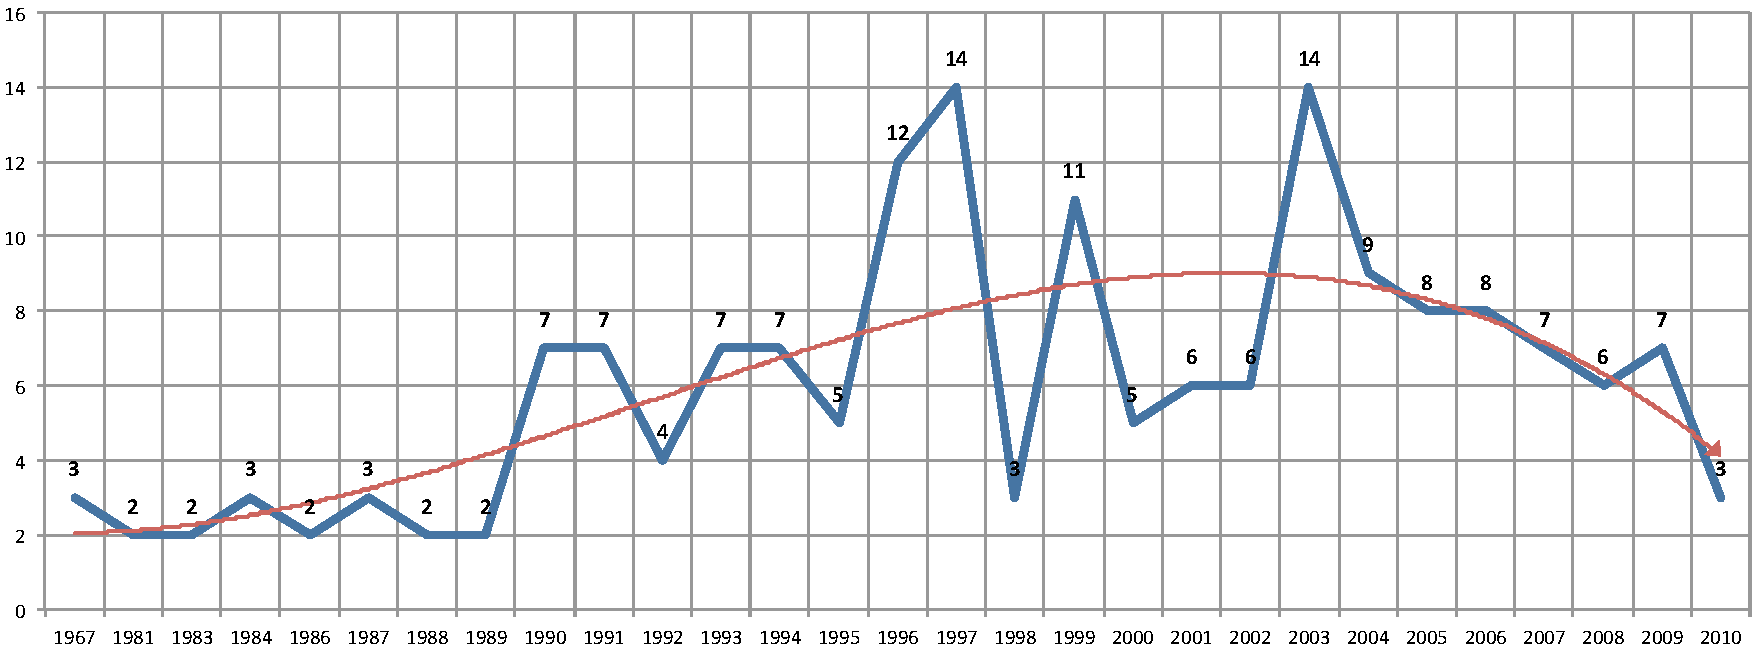
\includegraphics[scale=0.2]{Imagens/abntex2-modelo-img-grafico.pdf}
    \legend{Fonte: \citeonline[p. 24]{araujo2012}}
  \end{minipage}
\end{figure}

Observe que, segundo a \citeonline[seções 4.2.1.10 e 5.8]{NBR14724:2011}, as
ilustrações devem sempre ter numeração contínua e única em todo o documento:

\begin{citacao}
Qualquer que seja o tipo de ilustração, sua identificação aparece na parte
superior, precedida da palavra designativa (desenho, esquema, fluxograma,
fotografia, gráfico, mapa, organograma, planta, quadro, retrato, figura,
imagem, entre outros), seguida de seu número de ordem de ocorrência no texto,
em algarismos arábicos, travessão e do respectivo título. Após a ilustração, na
parte inferior, indicar a fonte consultada (elemento obrigatório, mesmo que
seja produção do próprio autor), legenda, notas e outras informações
necessárias à sua compreensão (se houver). A ilustração deve ser citada no
texto e inserida o mais próximo possível do trecho a que se
refere. \cite[seções 5.8]{NBR14724:2011}
\end{citacao}

% ---
\section{Expressões matemáticas}
% ---

\index{expressões matemáticas}Use o ambiente \texttt{equation} para escrever
expressões matemáticas numeradas:

\begin{equation}
  \forall x \in X, \quad \exists \: y \leq \epsilon
\end{equation}

Escreva expressões matemáticas entre \$ e \$, como em $ \lim_{x \to \infty}
\exp(-x) = 0 $, para que fiquem na mesma linha.

Também é possível usar colchetes para indicar o início de uma expressão
matemática que não é numerada.

\[
\left|\sum_{i=1}^n a_ib_i\right|
\le
\left(\sum_{i=1}^n a_i^2\right)^{1/2}
\left(\sum_{i=1}^n b_i^2\right)^{1/2}
\]

Consulte mais informações sobre expressões matemáticas em
\url{https://github.com/abntex/abntex2/wiki/Referencias}.

% ---
\section{Enumerações: alíneas e subalíneas}
% ---

\index{alíneas}\index{subalíneas}\index{incisos}Quando for necessário enumerar
os diversos assuntos de uma seção que não possua título, esta deve ser
subdividida em alíneas \cite[4.2]{NBR6024:2012}:

\begin{alineas}

  \item os diversos assuntos que não possuam título próprio, dentro de uma mesma
  seção, devem ser subdivididos em alíneas; 
  
  \item o texto que antecede as alíneas termina em dois pontos;
  \item as alíneas devem ser indicadas alfabeticamente, em letra minúscula,
  seguida de parêntese. Utilizam-se letras dobradas, quando esgotadas as
  letras do alfabeto;

  \item as letras indicativas das alíneas devem apresentar recuo em relação à
  margem esquerda;

  \item o texto da alínea deve começar por letra minúscula e terminar em
  ponto-e-vírgula, exceto a última alínea que termina em ponto final;

  \item o texto da alínea deve terminar em dois pontos, se houver subalínea;

  \item a segunda e as seguintes linhas do texto da alínea começa sob a
  primeira letra do texto da própria alínea;
  
  \item subalíneas \cite[4.3]{NBR6024:2012} devem ser conforme as alíneas a
  seguir:

  \begin{alineas}
     \item as subalíneas devem começar por travessão seguido de espaço;

     \item as subalíneas devem apresentar recuo em relação à alínea;

     \item o texto da subalínea deve começar por letra minúscula e terminar em
     ponto-e-vírgula. A última subalínea deve terminar em ponto final, se não
     houver alínea subsequente;

     \item a segunda e as seguintes linhas do texto da subalínea começam sob a
     primeira letra do texto da própria subalínea.
  \end{alineas}
  
  \item no \abnTeX\ estão disponíveis os ambientes \texttt{incisos} e
  \texttt{subalineas}, que em suma são o mesmo que se criar outro nível de
  \texttt{alineas}, como nos exemplos à seguir:
  
  \begin{incisos}
    \item \textit{Um novo inciso em itálico};
  \end{incisos}
  
  \item Alínea em \textbf{negrito}:
  
  \begin{subalineas}
    \item \textit{Uma subalínea em itálico};
    \item \underline{\textit{Uma subalínea em itálico e sublinhado}}; 
  \end{subalineas}
  
  \item Última alínea com \emph{ênfase}.
  
\end{alineas}

% ---
\section{Espaçamento entre parágrafos e linhas}
% ---

\index{espaçamento!dos parágrafos}O tamanho do parágrafo, espaço entre a margem
e o início da frase do parágrafo, é definido por:

\begin{verbatim}
   \setlength{\parindent}{1.3cm}
\end{verbatim}

\index{espaçamento!do primeiro parágrafo}Por padrão, não há espaçamento no
primeiro parágrafo de cada início de divisão do documento
(\autoref{sec-divisoes}). Porém, você pode definir que o primeiro parágrafo
também seja indentado, como é o caso deste documento. Para isso, apenas inclua o
pacote \textsf{indentfirst} no preâmbulo do documento:

\begin{verbatim}
   \usepackage{indentfirst}      % Indenta o primeiro parágrafo de cada seção.
\end{verbatim}

\index{espaçamento!entre os parágrafos}O espaçamento entre um parágrafo e outro
pode ser controlado por meio do comando:

\begin{verbatim}
  \setlength{\parskip}{0.2cm}  % tente também \onelineskip
\end{verbatim}

\index{espaçamento!entre as linhas}O controle do espaçamento entre linhas é
definido por:

\begin{verbatim}
  \OnehalfSpacing       % espaçamento um e meio (padrão); 
  \DoubleSpacing        % espaçamento duplo
  \SingleSpacing        % espaçamento simples	
\end{verbatim}

Para isso, também estão disponíveis os ambientes:

\begin{verbatim}
  \begin{SingleSpace} ...\end{SingleSpace}
  \begin{Spacing}{hfactori} ... \end{Spacing}
  \begin{OnehalfSpace} ... \end{OnehalfSpace}
  \begin{OnehalfSpace*} ... \end{OnehalfSpace*}
  \begin{DoubleSpace} ... \end{DoubleSpace}
  \begin{DoubleSpace*} ... \end{DoubleSpace*} 
\end{verbatim}

Para mais informações, consulte \citeonline[p. 47-52 e 135]{memoir}.

% ---
\section{Inclusão de outros arquivos}\label{sec-include}
% ---

É uma boa prática dividir o seu documento em diversos arquivos, e não
apenas escrever tudo em um único. Esse recurso foi utilizado neste
documento. Para incluir diferentes arquivos em um arquivo principal,
de modo que cada arquivo incluído fique em uma página diferente, utilize o
comando:

\begin{verbatim}
   \include{documento-a-ser-incluido}      % sem a extensão .tex
\end{verbatim}

Para incluir documentos sem quebra de páginas, utilize:

\begin{verbatim}
   \input{documento-a-ser-incluido}      % sem a extensão .tex
\end{verbatim}

% ---
\section{Compilar o documento \LaTeX}
% ---

Geralmente os editores \LaTeX, como o
TeXlipse\footnote{\url{http://texlipse.sourceforge.net/}}, o
Texmaker\footnote{\url{http://www.xm1math.net/texmaker/}}, entre outros,
compilam os documentos automaticamente, de modo que você não precisa se
preocupar com isso.

No entanto, você pode compilar os documentos \LaTeX usando os seguintes
comandos, que devem ser digitados no \emph{Prompt de Comandos} do Windows ou no
\emph{Terminal} do Mac ou do Linux:

\begin{verbatim}
   pdflatex ARQUIVO_PRINCIPAL.tex
   bibtex ARQUIVO_PRINCIPAL.aux
   makeindex ARQUIVO_PRINCIPAL.idx 
   makeindex ARQUIVO_PRINCIPAL.nlo -s nomencl.ist -o ARQUIVO_PRINCIPAL.nls
   pdflatex ARQUIVO_PRINCIPAL.tex
   pdflatex ARQUIVO_PRINCIPAL.tex
\end{verbatim}

% ---
\section{Remissões internas}
% ---

Ao nomear a \autoref{tab-nivinv} e a \autoref{fig_circulo}, apresentamos um
exemplo de remissão interna, que também pode ser feita quando indicamos o
\autoref{cap_exemplos}, que tem o nome \emph{\nameref{cap_exemplos}}. O número
do capítulo indicado é \ref{cap_exemplos}, que se inicia à
\autopageref{cap_exemplos}\footnote{O número da página de uma remissão pode ser
obtida também assim:
\pageref{cap_exemplos}.}.
Veja a \autoref{sec-divisoes} para outros exemplos de remissões internas entre
seções, subseções e subsubseções.

O código usado para produzir o texto desta seção é:

\begin{verbatim}
Ao nomear a \autoref{tab-nivinv} e a \autoref{fig_circulo}, apresentamos um
exemplo de remissão interna, que também pode ser feita quando indicamos o
\autoref{cap_exemplos}, que tem o nome \emph{\nameref{cap_exemplos}}. O número
do capítulo indicado é \ref{cap_exemplos}, que se inicia à
\autopageref{cap_exemplos}\footnote{O número da página de uma remissão pode ser
obtida também assim:
\pageref{cap_exemplos}.}.
Veja a \autoref{sec-divisoes} para outros exemplos de remissões internas entre
seções, subseções e subsubseções.
\end{verbatim}

% ---
\section{Divisões do documento: seção}\label{sec-divisoes}
% ---

Esta seção testa o uso de divisões de documentos. Esta é a
\autoref{sec-divisoes}. Veja a \autoref{sec-divisoes-subsection}.

\subsection{Divisões do documento: subseção}\label{sec-divisoes-subsection}

Isto é uma subseção. Veja a \autoref{sec-divisoes-subsubsection}, que é uma
\texttt{subsubsection} do \LaTeX, mas é impressa chamada de ``subseção'' porque
no Português não temos a palavra ``subsubseção''.

\subsubsection{Divisões do documento: subsubseção}
\label{sec-divisoes-subsubsection}

Isto é uma subsubseção.

\subsubsection{Divisões do documento: subsubseção}

Isto é outra subsubseção.

\subsection{Divisões do documento: subseção}\label{sec-exemplo-subsec}

Isto é uma subseção.

\subsubsection{Divisões do documento: subsubseção}

Isto é mais uma subsubseção da \autoref{sec-exemplo-subsec}.


\subsubsubsection{Esta é uma subseção de quinto
nível}\label{sec-exemplo-subsubsubsection}

Esta é uma seção de quinto nível. Ela é produzida com o seguinte comando:

\begin{verbatim}
\subsubsubsection{Esta é uma subseção de quinto
nível}\label{sec-exemplo-subsubsubsection}
\end{verbatim}

\subsubsubsection{Esta é outra subseção de quinto nível}\label{sec-exemplo-subsubsubsection-outro}

Esta é outra seção de quinto nível.


\paragraph{Este é um parágrafo numerado}\label{sec-exemplo-paragrafo}

Este é um exemplo de parágrafo nomeado. Ele é produzida com o comando de
parágrafo:

\begin{verbatim}
\paragraph{Este é um parágrafo nomeado}\label{sec-exemplo-paragrafo}
\end{verbatim}

A numeração entre parágrafos numeradaos e subsubsubseções são contínuas.

\paragraph{Esta é outro parágrafo numerado}\label{sec-exemplo-paragrafo-outro}

Esta é outro parágrafo nomeado.

% ---
\section{Este é um exemplo de nome de seção longo. Ele deve estar
alinhado à esquerda e a segunda e demais linhas devem iniciar logo abaixo da
primeira palavra da primeira linha}
% ---

Isso atende à norma \citeonline[seções de 5.2.2 a 5.2.4]{NBR14724:2011} 
 e \citeonline[seções de 3.1 a 3.8]{NBR6024:2012}.

% ---
\section{Diferentes idiomas e hifenizações}
\label{sec-hifenizacao}
% ---

Para usar hifenizações de diferentes idiomas, inclua nas opções do documento o
nome dos idiomas que o seu texto contém. Por exemplo (para melhor
visualização, as opções foram quebras em diferentes linhas):

\begin{verbatim}
\documentclass[
	12pt,
	openright,
	twoside,
	a4paper,
	english,
	french,
	spanish,
	brazil
	]{abntex2}
\end{verbatim}

O idioma português-brasileiro (\texttt{brazil}) é incluído automaticamente pela
classe \textsf{abntex2}. Porém, mesmo assim a opção \texttt{brazil} deve ser
informada como a última opção da classe para que todos os pacotes reconheçam o
idioma. Vale ressaltar que a última opção de idioma é a utilizada por padrão no
documento. Desse modo, caso deseje escrever um texto em inglês que tenha
citações em português e em francês, você deveria usar o preâmbulo como abaixo:

\begin{verbatim}
\documentclass[
	12pt,
	openright,
	twoside,
	a4paper,
	french,
	brazil,
	english
	]{abntex2}
\end{verbatim}

A lista completa de idiomas suportados, bem como outras opções de hifenização,
estão disponíveis em \citeonline[p.~5-6]{babel}.

Exemplo de hifenização em inglês\footnote{Extraído de:
\url{http://en.wikibooks.org/wiki/LaTeX/Internationalization}}:

\begin{otherlanguage*}{english}
\textit{Text in English language. This environment switches all language-related
definitions, like the language specific names for figures, tables etc. to the other
language. The starred version of this environment typesets the main text
according to the rules of the other language, but keeps the language specific
string for ancillary things like figures, in the main language of the document.
The environment hyphenrules switches only the hyphenation patterns used; it can
also be used to disallow hyphenation by using the language name
`nohyphenation'.}
\end{otherlanguage*}

O idioma geral do texto por ser alterado como no exemplo seguinte:

\begin{verbatim}
  \selectlanguage{english}
\end{verbatim}

Isso altera automaticamente a hifenização e todos os nomes constantes de
referências do documento para o idioma inglês. Consulte o manual da classe
\cite{abntex2classe} para obter orientações adicionais sobre internacionalização de
documentos produzidos com \abnTeX.

A \autoref{sec-citacao} descreve o ambiente \texttt{citacao} que pode receber
como parâmetro um idioma a ser usado na citação.

% ---
\section{Consulte o manual da classe \textsf{abntex2}}
% ---

Consulte o manual da classe \textsf{abntex2} \cite{abntex2classe} para uma
referência completa das macros e ambientes disponíveis. 

Além disso, o manual possui informações adicionais sobre as normas ABNT
observadas pelo \abnTeX\ e considerações sobre eventuais requisitos específicos
não atendidos, como o caso da \citeonline[seção 5.2.2]{NBR14724:2011}, que
especifica o espaçamento entre os capítulos e o início do texto, regra
propositalmente não atendida pelo presente modelo.

% ---
\section{Referências bibliográficas}
% ---

A formatação das referências bibliográficas conforme as regras da ABNT são um
dos principais objetivos do \abnTeX. Consulte os manuais
\citeonline{abntex2cite} e \citeonline{abntex2cite-alf} para obter informações
sobre como utilizar as referências bibliográficas.

%-
\subsection{Acentuação de referências bibliográficas}
%-

Normalmente não há problemas em usar caracteres acentuados em arquivos
bibliográficos (\texttt{*.bib}). Porém, como as regras da ABNT fazem uso quase
abusivo da conversão para letras maiúsculas, é preciso observar o modo como se
escreve os nomes dos autores. Na ~\autoref{tabela-acentos} você encontra alguns
exemplos das conversões mais importantes. Preste atenção especial para `ç' e `í'
que devem estar envoltos em chaves. A regra geral é sempre usar a acentuação
neste modo quando houver conversão para letras maiúsculas.

\begin{table}[htbp]
\caption{Tabela de conversão de acentuação.}
\label{tabela-acentos}

\begin{center}
\begin{tabular}{ll}\hline\hline
acento & \textsf{bibtex}\\
à á ã & \verb+\`a+ \verb+\'a+ \verb+\~a+\\
í & \verb+{\'\i}+\\
ç & \verb+{\c c}+\\
\hline\hline
\end{tabular}
\end{center}
\end{table}


% ---
\section{Precisa de ajuda?}
% ---

Consulte a FAQ com perguntas frequentes e comuns no portal do \abnTeX:
\url{https://github.com/abntex/abntex2/wiki/FAQ}.

Inscreva-se no grupo de usuários \LaTeX:
\url{http://groups.google.com/group/latex-br}, tire suas dúvidas e ajude
outros usuários.

Participe também do grupo de desenvolvedores do \abnTeX:
\url{http://groups.google.com/group/abntex2} e faça sua contribuição à
ferramenta.

% ---
\section{Você pode ajudar?}
% ---

Sua contribuição é muito importante! Você pode ajudar na divulgação, no
desenvolvimento e de várias outras formas. Veja como contribuir com o \abnTeX\
em \url{https://github.com/abntex/abntex2/wiki/Como-Contribuir}.

% ---
\section{Quer customizar os modelos do \abnTeX\ para sua instituição ou universidade?}
% ---

Veja como customizar o \abnTeX\ em: \\
\url{https://github.com/abntex/abntex2/wiki/ComoCustomizar}.
% \chapter{Conteúdos específicos do modelo de trabalho acadêmico}\label{cap_trabalho_academico}

\section{Quadros}

Este modelo vem com o ambiente \texttt{quadro} e impressão de Lista de quadros 
configurados por padrão. Verifique um exemplo de utilização:

\begin{quadro}[htb]
\caption{\label{quadro_exemplo}Exemplo de quadro}
\begin{tabular}{|c|c|c|c|}
	\hline
	\textbf{Pessoa} & \textbf{Idade} & \textbf{Peso} & \textbf{Altura} \\ \hline
	Marcos & 26    & 68   & 178    \\ \hline
	Ivone  & 22    & 57   & 162    \\ \hline
	...    & ...   & ...  & ...    \\ \hline
	Sueli  & 40    & 65   & 153    \\ \hline
\end{tabular}
\fonte{Autor.}
\end{quadro}

Este parágrafo apresenta como referenciar o quadro no texto, requisito
obrigatório da ABNT. 
Primeira opção, utilizando \texttt{autoref}: Ver o \autoref{quadro_exemplo}. 
Segunda opção, utilizando  \texttt{ref}: Ver o Quadro \ref{quadro_exemplo}.
% % ---
% Capitulo de revisão de literatura
% ---
\chapter{Lorem ipsum dolor sit amet}
% ---

% ---
\section{Aliquam vestibulum fringilla lorem}
% ---

\lipsum[1]

\lipsum[2-3]

% ---
% primeiro capitulo de Resultados
% ---
\chapter{Lectus lobortis condimentum}
% ---

% ---
\section{Vestibulum ante ipsum primis in faucibus orci luctus et ultrices
posuere cubilia Curae}
% ---

\lipsum[21-22]

% ---
% segundo capitulo de Resultados
% ---
\chapter{Nam sed tellus sit amet lectus urna ullamcorper tristique interdum
elementum}
% ---

% ---
\section{Pellentesque sit amet pede ac sem eleifend consectetuer}
% ---

\lipsum[24]
% \chapter{Customização DCOMP}

\section{Lista de códigos}

Usado para criar a lista de códigos, adicionar sintaxe highlight, enumerar as linhas e colorir o fundo, para dar destaque a implementação.

Sintaxe básica:
\begin{verbatim}
\begin{codigo}[!htb]
    \caption{Espaço para o título do código}
    \label{Espaço para o label do código, para ser usado na referência}  
    \begin{lstlisting}[language = Linguagem de programação a ser usada]
        <CÓDIGO>
    \end{lstlisting}
\end{codigo}
\end{verbatim}

\begin{codigo}[htb]
  \caption{Código PHP}
  \label{codigophp}
  \begin{lstlisting}[language = php]
       <?php

       echo '%*Olá mundo*)!';
       print '%*Olá mundo*)!';
  \end{lstlisting}
\end{codigo}

\begin{codigo}
  \caption{Código python}
  \label{codigopython}
  \begin{lstlisting}[language = python]
    import numpy as np
 
    def incmatrix(genl1, genl2):
        m = len(genl1)
        n = len(genl2)
        M = None #to become the incidence matrix
        VT = np.zeros((n*m,1), int)  #dummy variable
 
        #compute the bitwise xor matrix
        M1 = bitxormatrix(genl1)
        M2 = np.triu(bitxormatrix(genl2),1) 
 
        for i in range(m-1):
            for j in range(i+1, m):
                [r,c] = np.where(M2 == M1[i,j])
                for k in range(len(r)):
                    VT[(i)*n + r[k]] = 1;
                    VT[(i)*n + c[k]] = 1; 
                    VT[(j)*n + r[k]] = 1;
                    VT[(j)*n + c[k]] = 1;
 
                    if M is None:
                        M = np.copy(VT)
                    else:
                        M = np.concatenate((M, VT), 1)
 
                    VT = np.zeros((n*m,1), int)
 
        return M
\end{lstlisting}
\end{codigo}

\begin{codigo}
  \caption{Codigo Java}
  \begin{lstlisting}[language = Java]
    public class Factorial{
        public static void main(String[] args){   
            final int NUM_FACTS = 100;
            for(int i = 0; i < NUM_FACTS; i++)
                System.out.println( i + "! is " + factorial(i) + factorial(i) factorial(i) factorial(i));
        }

        public static int factorial(int n){
            int result = 1;
            for(int i = 2; i <= n; i++)
                result *= i;
            return result;
        }
    }
\end{lstlisting}
\end{codigo}



\section{Lista de Algoritmos}

Usado para criar a lista de algoritmos ou pseudocodigos.

Sintaxe básica:
\begin{verbatim}
\begin{algoritmo}[!htb]
    \caption{Espaço para o título do algoritmo ou pseudocodigo}
    \label{label do do algoritmo ou pseudocodigo, para ser usado na referência}  
    <ESPAÇO RESERVADO PARA USAR SEU PACOTE FAVORITO DE CÓDIGOS>
\end{algoritmo}
\end{verbatim}


\begin{algoritmo}[htb]
	\caption{Algoritmo exemplo}
	\label{alg1}
	\begin{algorithm}[H]
 	\KwData{this text}
 	\KwResult{how to write algorithm with \LaTeX2e }
 	initialization\;
 	\While{not at end of this document}{
  		read current\;
  		\eIf{understand}{
   			go to next section\;
   			current section becomes this one\;
   		}{
   			go back to the beginning of current section\;
  		}
 	}
	\end{algorithm}
\end{algoritmo}

% \chapter{Conclusão}\label{chapter-conclusao}

As conclusões constituem a parte final do texto, na qual se apresentam as considerações finais sobre o assunto, se os objetivos foram alcançados, o que se descobriu, quais outras questões surgiram a partir dos resultados e se as hipóteses se confirmaram ou não. Vale lembrar que nenhum trabalho de pesquisa encerra um tema ou problema, por isso, evite fazer afirmações redutoras ou definitivas.

\phantompart
\bibliography{Bibliografia}

%%%%%%%%%%%%%%%%%%%%%%%%%%%%%%%%%%%%%%%%%%%%%%%%%%%%%%%%%%%%%%%%%%%%%%%%%%
% ELEMENTOS PÓS-TEXTUAIS
%%%%%%%%%%%%%%%%%%%%%%%%%%%%%%%%%%%%%%%%%%%%%%%%%%%%%%%%%%%%%%%%%%%%%%%%%%

\postextual

\renewcommand{\chapnumfont}{\chaptitlefont}
\renewcommand{\afterchapternum}{}
\include{Pos_Textual/Apendices}
\include{Pos_Textual/Anexos}

\end{document}
